\documentclass{article}
\usepackage[utf8]{inputenc}
\usepackage[T1]{fontenc}
\usepackage{scrextend}
\usepackage{gensymb}
\usepackage{graphicx}
\graphicspath{ {./img/procedure/}{./img/results/} }
\title{Master Thesis}
\author{Marcel Bechtold}
\date{July 2018}


\begin{document}

\maketitle


\section{Abstract}

Lorem ipsum

\section{Introduction}


\section{Methods}

\subsection{Participants}
Twenty participants(10 female, 10 male; all right-handed) from the local university community participated in the experiment. Their age ranged from XX to XX years (M = XX, SD = XX). All participants were naive to the purpose of the experiment and had normal or corrected-to-normal vision. The experiment was approved by the ethics committee of the University of T\"ubingen, and was performed in accordance with the Declaration of Helsinki. Participants gave written informed consent prior to the experiment and were compensated with 8 Euro per hour for their participation. 

\subsection{Apparatus}
The virtual environment was displayed in stereo using an HTC Vive head-mounted-display (HMD) with a resolution of 1080 x 1200 pixels per eye (2160 x 1200 pixels combined). Inter-pupillary distance was measured with a pupilometer and set accoringly on the HTC Vive for each participant. Audio was recorded with a microphone plugged into the integrated audio input of the HTC Vive. Participants were standing during the whole experiment and viewed their virtual task in front of them.

Participants were run in an individual and a collaborative condition in which two participants worked together. Therefore the apparatus consisted of two HTC Vives of which each was connected to its own computer. The computers had the same hardware configuration (list PC specs?). In the individual condition participants were run in their own virtual environment solving a task alone (\ref{fig:individual_condition_setting}). In the collaborative condition two participants were run in a shared virtual environment solving the task together (\ref{fig:collaborative_condition_setting}). The synchronization between the two computers in the collaborative condition was done via UDP. Therefore the participants could collaborate in real time with very little to no delay or lag.

The virtual task consists of cubes and cube slots. The cubes can be picked up by moving the controller into a cube and pressing and holding the trigger button of the controller (there is both no collision between cubes and between cubes and the controller). When a cube is picked up it can be moved and rotated freely by the controller. When the cube is moved to the solution space it  automatically aligns ("snaps in") with the next closest cube slot.

%\begin{figure}
%\centering
%\includegraphics[width=0.8\textwidth]{individual_condition_setting.png}
%\caption{\label{fig:individual_condition_setting} XX.}
%\end{figure}

%\begin{figure}
%\centering
%\includegraphics[width=0.8\textwidth]{collaborative_condition_setting.png}
%\caption{\label{fig:collaborative_condition_setting} XX.}
%\end{figure}




\subsection{Task Design}
Participants were invited as a group of two people and did not know each other. In one group session the two participants solved the task on their own in a separate virtual environment and together in the same virtual environment. The sequence of single and collaborative was counter balanced among all groups. In both the single and collaborative condition participants solved 20 tasks of which all had the same design as described above and differed only in color. In the single condition participants viewed the task always from the same perspective, which means that the starting cube was always placed at the same position in the solution space.
In the collaborative condition we rotated the solution space after 10 trials, which means the starting cube is on one participant's side for the first 10 trials and on the other participant's side for the remaining 10 trials. 

The detailed procedure for the single condition will be explained in the following:
After having read the instructions of the task participants also received a verbal instruction by the experimenter. Before the actual 20 trials began participants had to solve two training trials in order to verify that the participant understood the task and the way it has to be solved. It was emphasized that it is important to always stick to the sequence of putting in and removing cubes as described above. Furthermore participants could experience that the starting cube can not be removed and is the only cube in the experiment with which the other cubes collide (that was important because we wanted to avoid that cubes can be places so that they overlap with the starting cube). Participants could also get used to the fact that the top color is always white and the bottom color is always black. The training trials could be started by the participant by holding a controller button for 2 seconds. When they start the training they saw the solution space surrounded by the 9 cubes which are all in reaching distance. They also saw the starting cube already being placed into the solution space. Above the task participants could see in which trial they currently are. In this case they would see "Training 1/2". Once they have finished a trial they can proceed with the next trial by pressing the controller button again for 2 seconds. 

Before the actual 20 trials start the experimenter repeats the most important instructions.Participants should try to solve the task as quickly and as accurately as possible. Also that they are not allowed to move around the problem space and should stay mostly stationary in their position with only a few steps to the sides allowed.
After the two training trials participants could start the actual trials as soon as they were ready by clicking a controller button again for 2 seconds. For the actual trial the experimenter would emphasize that participants should always make sure their solution is correct before proceeding with the next task. In case participants did not correctly solve a task and still proceed with the next task the experimenter took note in order to exclude the trial from the analysis.

The procedure for the collaborative solving of the task was mostly the same. The only difference was that just one participant was able to skip to the next trial and therefore the instructions were that participants had to agree on when to proceed with the next task.

%what needs to go in here is:

%instructions that were given to the participants
%training phase (how many trials...)
%counterbalance single / multi (counterbalanced - 10 each side)

\section{Details about the task}

\subsection{Implications for problem solving}

\section{Results}
Data analysis was done by applying linear mixed models with the Kenward-Rodger degrees of freedom approximation. The random factors were the group number (= an individual number assigned to each group in the group condition), participant number (= an individual number assigned to each individual participant in the single condition) and the number of players(= either one or two). The only fixed factor was the number of players. 

 Although much more data has been recorded during the experiment this section will only cover the most relevant results that suit best to compare the performances of the single vs the group condition. 
 
 All data was automatically recorded from the time participants pressed the controller button to start the task to when they pressed the button again in order to skip to the next task. The data was based on the controller trajectories, rotations and user input  In the following the term "task duration" will be used to describe this duration in which data was recorded for an individual task.

\paragraph{Time to complete}
The time to complete is the average of all task durations.  Figure \ref{fig:results_duration} shows that the groups were much faster with an average of 50 seconds compared to single participants with an average of 80 seconds. The output of the linear mixed model was F:(1,18.99) = 52.049, p < 0.001 

\begin{figure}[h]
\centering
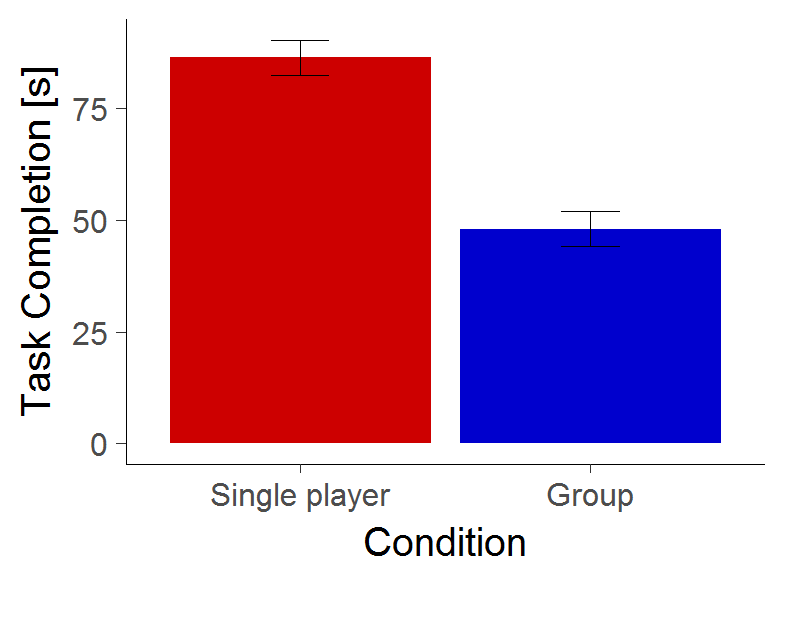
\includegraphics[width=0.5\textwidth]{results_duration}
\caption{Average time in seconds to complete the task in singel and group condition.} \label{fig:results_duration}
\end{figure}

\paragraph{Rotation sum of cubes}
The rotation sum of cubes is the sum of rotations made by one participant during the task duration. In the group condition we summed up the rotations of both group members first and calculated the averages over the group sums. Figure \ref{fig:results_rotations} shows that the average rotation sum for groups with an average of 5000 degrees was significantly less compared to single participants with an average of 8000 degrees. For the rotation sum a the smaller value indicates the better performance because the less a participant rotates a cube the more confident and efficient the participant is expected to be at solving the task. The output of the linear mixed model was F:(1,18.99) = 12.164, p < 0.01.

\begin{figure}[h]
\centering
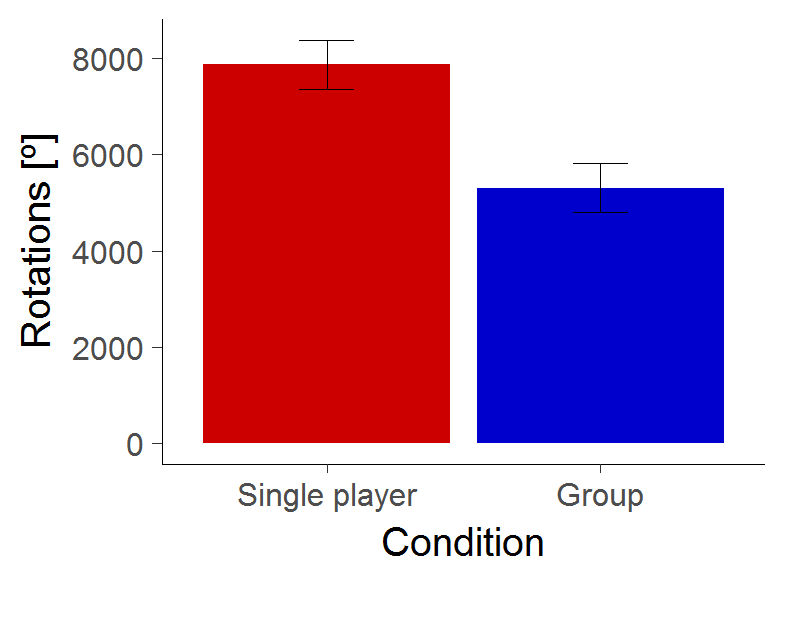
\includegraphics[width=0.5\textwidth]{results_rotations}
\caption{Sum of rotations in degrees.}
\label{fig:results_rotations}
\end{figure}

\paragraph{Number of cube snap-outs}
The number of cube snap-outs it the number of how many times a participant took a cube back out from the problem space during the task duration. Figure \ref{fig:results_snap_outs} shows that groups needed much less snap-outs with an average of 2.1 snap-outs compared to single participants with an average of 4.5 snap-outs. 

Snap-outs can be categorized in two classes: "necessary" and "unnecessary" snap-outs. Necessary snap-outs are the ones which are part of the task design which means participants are supposed to try certain solution paths and if a path was not successful they need to snap-out some cubes and snap-in new ones until they successfully finish the task. It is possible though that participants try the same or similar solution path more than one time and therefore have to do unnecessary snap-outs. For the number of cube snap-outs a smaller value indicates the better performance, because it means that less unnecessary snap-out were made. The average of necessary snap-outs is expected to be equally distributed with an expectancy value of 2.0. In other words scoring an average of 2.0 snap-outs is an indicator of almost perfect performance to which the group condition is very close with 2.1.
The output of the linear mixed model was F:(1,18.99)=22.112, p < 0.001.

\begin{figure}[h]
\centering
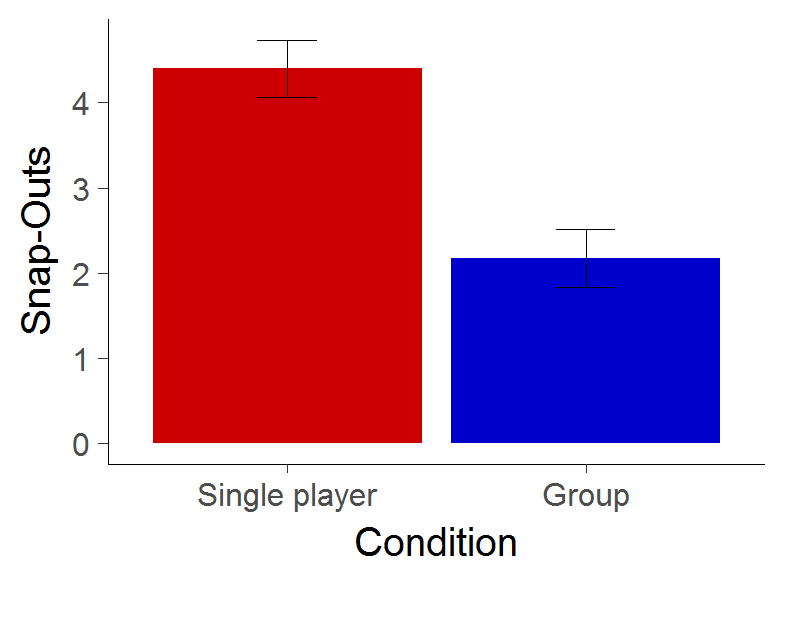
\includegraphics[width=0.5\textwidth]{results_snap_outs}
\caption{Example of a parametric }
\label{fig:results_snap_outs}
\end{figure}

\paragraph{Number of solution paths}

The output of the linear mixed model was F:(1,18.99)=4.565, p < 0.05.


\begin{figure}[h]
\centering
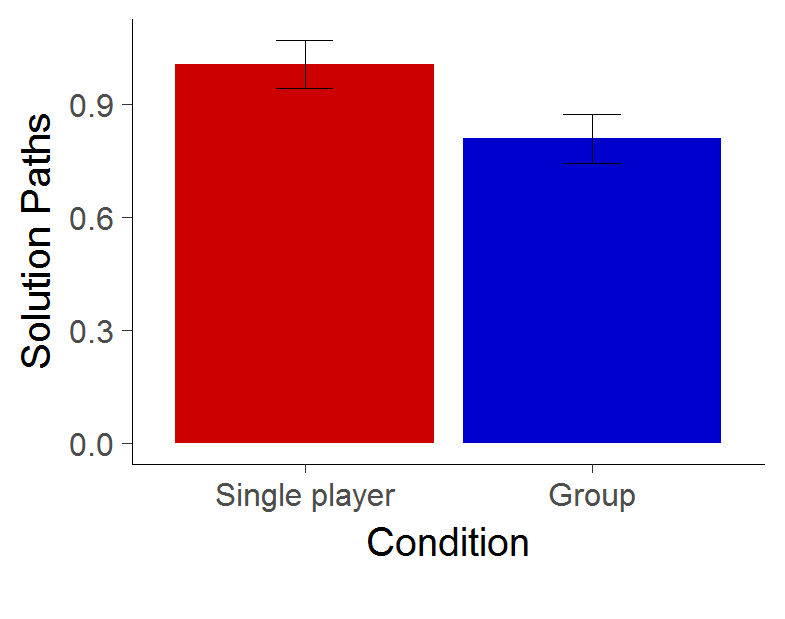
\includegraphics[width=0.5\textwidth]{results_solution_paths}
\caption{Example of a parametric }
\end{figure}

\paragraph{Error}

The output of the linear mixed model was F:(1,18.99)=9.338, p < 0.01.


\begin{figure}[h]
\centering
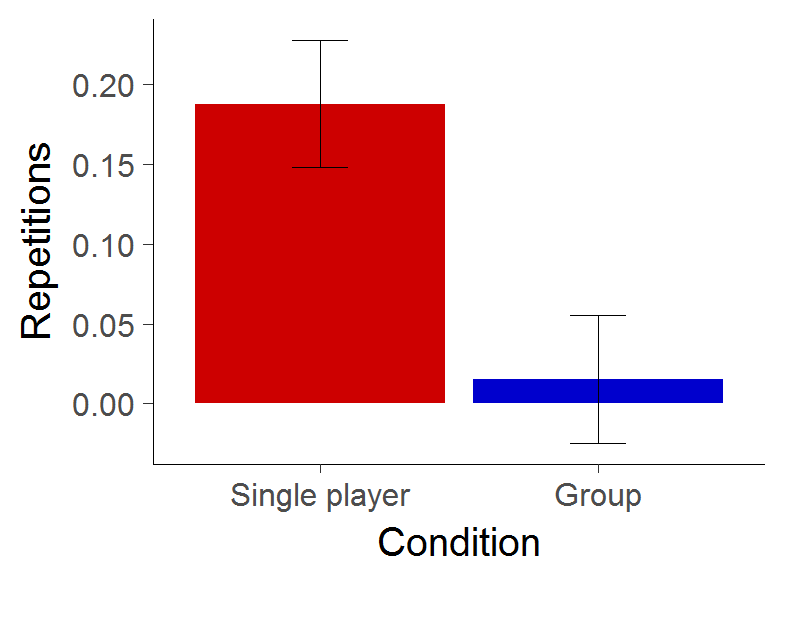
\includegraphics[width=0.5\textwidth]{results_un_error}
\caption{Example of a parametric }
\end{figure}


\section{Discussion}
Ideas behind the task design:
- very controlled: reduce the variation of how participants could solve the task
- tree like solution path: 
--four potential ways to traverse the tree in order to get to the solution
--best case one traversion, worst case four traversions
--how many traversions participants need is random and not controlled, but it is possible to quantify how close participants were to one certain traversion path and the deviation from that can be defined as the error.


\bibliography{references.bib}

\end{document}
